\chapter{Componenti di supporto a Sp[3]MM}
In questo capitolo verranno analizzati diversi componenti ausiliari
sviluppati ed integrati per supportare le operazioni di SpMM e Sp3MM.\\
%%%%%%%%%%%%%%%%%%%%%%  CORE  -- >> << -- xD  %%%%%%%%%%%%%%%%%%%%%%%%%%%%%%%%%%
\section[Derivazione di molteplici implementazioni con PreProcessore C]	
{Derivazione automatica di molteplici implementazioni mediante PreProcessore C}	\label{chSpMMAux:multiImpl}
Sfruttando una serie di direttive del pre processore C, sono riuscito ad ottenere
per molte funzioni scritte nei sorgenti, varie versioni differenti ottenute a tempo di pre-processamento, 
accessibili in altre funzioni mediante una segnatura modificata.\\
La necessità principale di realizzare questo approccio è stato quello di supportare, con
un'alta efficienza, l'integrazione del codice C in un progetto fortran come \cite{PSBLAS3},
come verrà trattato a breve in \ref{chSpMMAux:fortranIntegrate}.\\
%PRO GENERAL CPP MULTI VERSION IMPLEMENTATIONS
I vantaggi di usare il pre processore per ottenere molteplici versioni di una funzione sono diverse:
\begin{itemize}
	\item	la possibilità di escludere completamente sezioni di codice non utili ad una versione
	\item	la possibilità di aumentare di molto il riuso del codice scritto
	\item	rispetto ad incapsulare in sotto funzioni le differenze delle varie versioni da ottenere
			rispetto ad una funzione  base:
	\begin{itemize}
		\item	si consente al compilatore di effettuare ottimizzazioni 
				su ogni versione ottenuta in seguito al pre processamento, non possibili a run-time,
				come ad esempio semplificare un offset pari a zero da applicare ad operazioni di indicizzazione
				%(come ad esempio usare una diversa indicizzazione all'interno di un applicazione Fortran
				%\ref{chSpMMAux:fortanIdxsDifferent} )
		\item	evitare istruzioni di branching addizionali nel codice, (come analizzato in \ref{chSpMMSymb:funcsMultiImpleVSmanualMultiFunc} )
				che potenzialmente permettono ulteriori ottimizzazioni a tempo di compilazione.\\
	\end{itemize}
\end{itemize}
Ho pubblicato un semplice esempio di questo approccio implementativo in \url{https://github.com/andreadiiorio/C_Compile_Multi_Implementation_Automatically}.\\
\voidLine
Per ottenere diverse implementazioni da una funzione è necessario:
\begin{itemize}
	\item	racchiudere le differenze richieste da ogni versione in una funzione \emph{base o generica} con una serie di direttive \verb|#if ... #endif| ,\\
			così da consentire al preprocessore l'aggiunta del codice necessario a modificare la funzione base.%ad una particolare versione.
	\item	Le diverse versioni della funzione \emph{generica} devono essere esportate ad altre funzioni mediante una segnatura differente.\\
			Per questo è possibile aggiungere un  suffisso al nome ed eventualmente argomenti addizionali alla funzione 
			\emph{base}, mediante la concatenazione di stringhe del pre-processore C.\\
			Un possibile approccio per supportare la concatenazione di stringhe e macro di configurazione
			in questo contesto è quello di usare la macro \vvv{CAT} del seguente blocco di codice.\\
			\begin{lstlisting}
#define _STR(s) #s
#define STR(s) _STR(s)

//Concatenate preprocessor tokens A and B WITHOUT   expanding macro definitions
#define _CAT(a,b)    a ## b
//Concatenate preprocessor tokens A and B           EXPANDING macro definitions
#define CAT(a,b)    _CAT(a,b)
			\end{lstlisting}
	\item	Le funzioni generiche devono essere racchiuse in un sorgente dedicato, ed incluse da un altro mediante \verb|#include|,
			per un numero di volte pari al numero di versioni che è necessario ottenere,
			ridefininendo le macro ausiliare di configurazione delle implementazioni differenti.
	\item	per avere esportate le dichiarazioni delle versioni differenti realizzate, è possibile reiterare l'approccio 
			appena descrito agli header files.
\end{itemize}
 
\subsection{Supporto integrazione in progetto Fortran} \label{chSpMMAux:fortranIntegrate}
Al giorno d'oggi esistono vari approcci per integrare un applicazione C in una Fortran e viceversa,
grazie agli standard del linguaggio Fortran 2003 e 2018, come descritto in \cite{modernFortranExplained}.\\
Una differenza sostanziale di questi due linguaggi è l'uso di una differente indicizzazione, 
dove il C è a base 0 e il Fortran è a base 1.\\
%need double indexing generic
È necessario tenere a mente questa differenza dato che in ogni formato di memorizzazione sparso di matrici 
sono presenti degli indici relativi alla posizione dei valori \nnz nella matrice.\\
%efficient approch
Per supportare l'integrazione di questo lavoro in \cite{AMG4PSBLAS},
è stato necessario supportare efficientemente un passaggio tra l'indicizzazione
dell'applicazione fortran a quella C per eseguire il prodotto, eseguendo poi il vicerversa 
nel ritorno all'applicazione chiamante.\\
Al fine di supportare efficientemente il cambio di questi indici 
ho sfruttato l'approccio descritto per ottenere 2 versione per ogni funzione,
una che accetti l'indicizzazione nativa del C e un'altra che accetti l'indicizzazione del Fortran,
mediante l'aggiunta di un suffisso numerico ad ogni nome di funzione %.\\
come nell'esempio successivo.\\ 
\begin{lstlisting}
spmat* CAT(spmmRowByRow_SymbNum_,OFF_F)(spmat* A,spmat* B, CONFIG* cfg){...}
\end{lstlisting}
Dalla funzione precedente, definita nel file \verb|Sp3MM_CSR_OMP_Symb_Generic.c| per eseguire il prodotto numerico con un partizionamento del lavoro 1D 
verranno ottenute due versioni distinte per supportare le due indicizzazioni in base al valore della macro \verb|OFF_F| al momento
dell'inclusione del sorgente.\\
La doppia indicizzazione è realizzata dall'uso della macro \verb|OFF_F| all'interno della funzione 
come costante sottratta ad ogni indice preveniente dal Fortran prima di utilizzarlo per indicizzare un qualsiasi vettore,
ed avrà valore \vvv{1} nella versione da usare in un'applicazione Fortran o \vvv{0} per una applicazione C.\\
Un vantaggio immediato di avere una versione dedicata all'indicizzazione C è quello di avere la certezza 
quasi assoluta che la correzione degli indici con il valore \vvv{0} in \verb|OFF_F| verrà ottimizzata via dal compilatore.\\
%defined interface
Inoltre, per favorire una interoperabilità tra le varie implementazioni per le operazioni di SpMM e Sp3MM 
ho definito le seguenti interfacce per le operazioni:
\begin{lstlisting}
typedef spmat* (*SPMM_INTERF )  (spmat*,spmat*,CONFIG*);
typedef spmat* (*SP3MM_INTERF)  (spmat*,spmat*,spmat*,CONFIG*,SPMM_INTERF);
\end{lstlisting}
Dove \vvv{spmat} è una struttura con campi per supportare varie rappresentazioni sparse 
come CSR o ELL, mentre \vvv{CONFIG} contiene la configurazione per le esecuzioni delle operazioni in oggetto,
come ad esempio la griglia di parallelizzazione del lavoro o il numero di thread da utilizzare.\\

Per supportare il lato Fortran dell'integrazione è stato sfruttato il modulo \verb|iso_c_binding| 
per definire le interfacce e strutture con controparte nel codice C, in un modulo di supporto.\\

\subsection{Generazione efficiente di diverse versioni di una funzione base}	\label{chSpMMAux:multiImplMany}
Estendendo la soluzione appena riportata per generare una coppia di implementazioni per gestire una doppia indicizzazione,
ho realizzato un supporto alla generazione di otto versioni differenti di una funzione generica nel modulo relativo al prodotto simbolico.\\
Per realizzare le varie combinazioni di versioni richieste di ogni funzione per generare i vari livelli di dettaglio dell'output 
del prodotto simbolico descritti in \ref{chSpMMSymb:outputDetailLevel_coreFuncsVersions},
ho usato il seguente approccio basato su redefinizioni di alcune macro di supporto:\\
\begin{lstlisting}
#define OFF_F 0
	///generate basic versions
	#include "Sp3MM_CSR_OMP_SymbStep_Generic.c"
	///generate outIdxs versions
	#define OUT_IDXS 	OUT_IDXS_ON	
		#include "Sp3MM_CSR_OMP_SymbStep_Generic.c"
	#undef  OUT_IDXS
	///generate colParts versions
	#define COL_PARTS	COL_PARTS_ON
		#include "Sp3MM_CSR_OMP_SymbStep_Generic.c"
		//generate outIdxs AND colParts versions
		#define OUT_IDXS 	OUT_IDXS_ON
		#include "Sp3MM_CSR_OMP_SymbStep_Generic.c"

	#undef OUT_IDXS
	#undef COL_PARTS
#undef OFF_F
#define OFF_F 1
...
\end{lstlisting}
Nel frammento di codice precedente vengono generate dal preprocessore C otto diverse versioni
della maggior parte delle funzioni definite nel sorgente \\ \verb|Sp3MM_CSR_OMP_SymbStep_Generic.c|
combinando la ridefinizione delle macro di configurazione \verb|OUT_IDXS COL_PARTS OFF_F|.\\

\section{Linux Kernel 5.10.85 RedBlack Tree Userspace porting} \label{chSpMMAux:linuxRBTree}
L'implementazione dei RedBlack Tree usati nel prodotto simbolico è ottenuta effettuando un porting in 
userspace dei moduli relativi del kernel Linux 5.10.85.\\
\subsection{RedBlack nel kernel Linux}
\begin{figure}[H]
  \centering 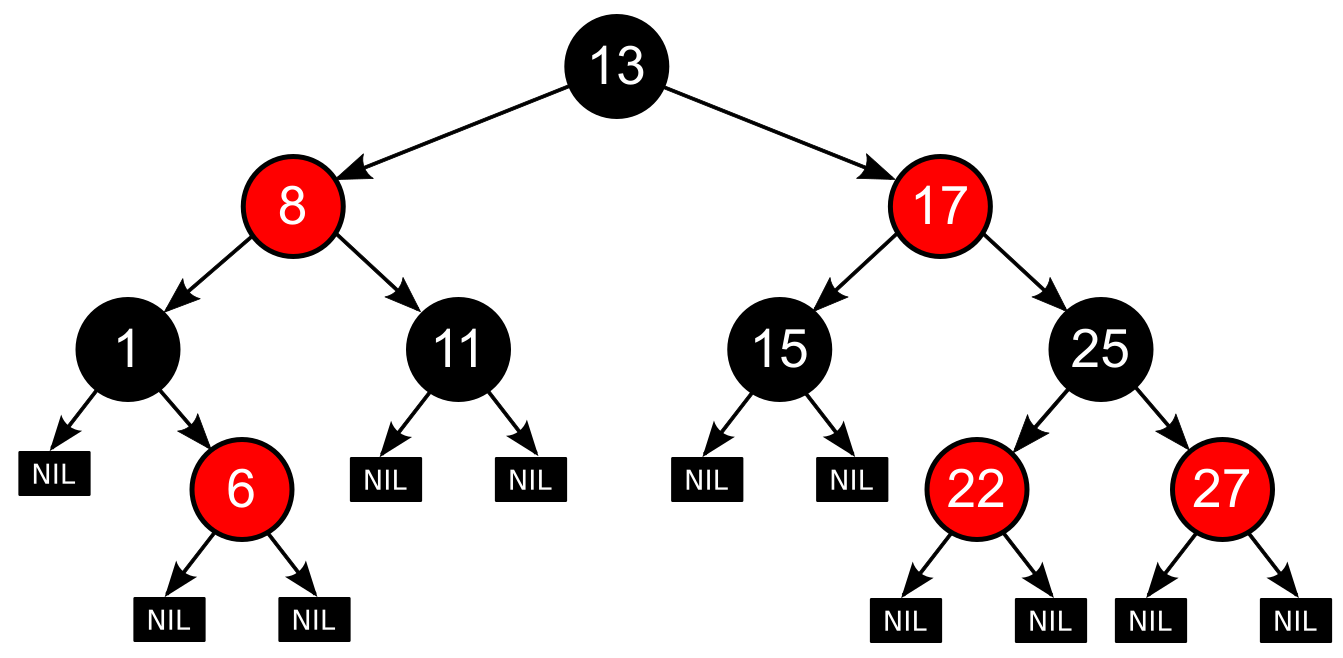
\includegraphics[width=.7\linewidth,keepaspectratio]{Red-black_tree_example.svg.pdf}
  \caption{Rappresentazione grafica di un RedBlack Tree}
  \decoRule \label{fig:rbtree}
\end{figure}
I RedBlack Tree sono delle strutture di ricerca molto efficienti catalogabili come 
\emph{Alberi binari auto bilanciati}.\\%self//semi-balancing binary search tree
La loro formulazione comprende diversi vincoli strutturali, da mantenre in seguito ad ogni operazione di inserimento o cancellazione,
che garantiscono ottime proprietà di bilanciamento tra cui avere che:\\ %| path: root ⟶ foglia più lontana | ≤  2* | path: root ⟶ foglia più vicina |
la distanza tra la radice dell'albero e la foglia più lontana è minore o uguale della distanza tra la radice e la foglia più vicina.\\
Le proprietà di bilanciamento assieme ai vincoli strutturali garantiscono ai RedBlack Tree
un costo computazione logaritmico al numero di elementi inseriti per ogni operazione.\\
\voidLine
Il kernel del sistema operativo Linux usa i RedBlack Tree per vari scopi, tra cui:
\begin{itemize}
	\item	le regioni di memoria virtuale (VMAs) associate ad un processo
	\item	la gestione delle directory nel filesystem ext3
	\item	la gestione dei timer ad alta risoluzione attivi
	\item	la gestione dei pacchetti di rete nello scheduler \vvv{hierarchical token bucket}
	\item	il tracciamento delle richieste negli schedulers \verb|CFQ I/O| e \vvv{deadline}
	\item	la gestione dei pacchetti nel driver per CD/DVD
	\item	la gestione degli epoll file descriptors
	\item	la gestione delle chiavi crittografiche
\end{itemize}  
\cite{lwnAgumentedRBtrees,lwnRBtrees}
\voidLine
\label{chSpMMAux:memRegionRBTree}
Un esempio dell'importanza dei RedBlack Tree è il primo punto della lista precedente,
ovvero la gestione degli indirizzi associati ad un processo Linux.\\\
Lo spazio degli indirizzi di memoria virtuale di un processo in Linux è implementato mediante una serie
di intervalli di indirizzi denominati regioni di memoria, salvati sia in una lista collegata che in un RedBlack, contenuti
nel \vvv{Memory Descriptor} di un processo.\\
Per supportare una ricerca efficiente della regione di memoria associata o vicina ad un indirizzo
(e.g. \verb|find_vma( )| ) viene usato il RedBlack tree, 
mentre per operazioni di scansione completa dello spazio degli indirizzi viene utilizzata la lista collegata
\cite{ulk}.\\
\voidLine
Segue una rappresentazione schematica delle strutture relative alla gestione delle regioni di memoria, con
un focus sui RedBlack 
\begin{figure}[H]
  \centering 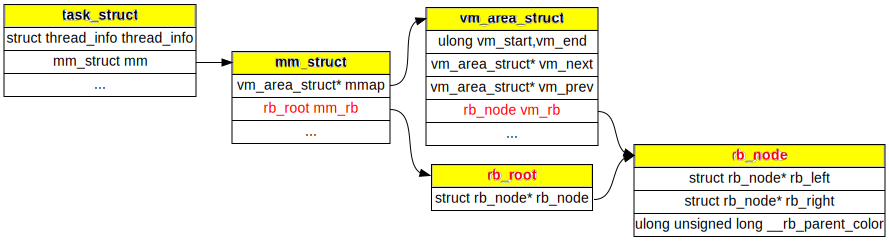
\includegraphics[width=.7\linewidth,keepaspectratio]{RBtreeInMMDesriptor.dot.colored.svg.pdf}
  \caption[RedBlackTree nella gestione degli address space in Linux]
  {Rappresentazione delle strutture usate per la gestione dello spazio degli indirizzi di un processo
			evidenziando la presenza dei RedBlack Tree}
  \decoRule \label{fig:RBtreeInMMDesriptor}
\end{figure}
Nella figura precedente è evidenziato come da un processo \vvv{p}(\verb|task_struct|) è possibile
accedere al suo \vvv{Memory Descriptor} associato (\verb|mm_struct|), contente le varie 
regioni di memoria (\verb|vm_area_struct|) relative ai vari intervalli di indirizzi 
collegati a \vvv{p}.\\
La gestione delle regioni di memoria è possibile sia mediante la strutturazione degli stessi 
in lista collegata (campi \verb|vm_next vm_prev| in \verb|vm_area_struct|),
sia mediante RedBlack tree grazie ai campi evidenziati in rosso in \ref{fig:RBtreeInMMDesriptor}
\voidLine
Dalle strutture \verb|rb_root rb_node| dei RedBlack appena mostrate è possibile notare l'assenza 
campi contenenti chiavi o puntatori a strutture nodo. 
Questo fatto è dovuto alla scelta di ottimizzare l'implementazione di queste strutture eliminando 
layers di indirezione inutili all'esecuzione delle funzionalità principali di questi alberi.
Da questa scelta degli sviluppati del kernel linux consegue la necessità di dover 
innestare le strutture \verb|rb_node| all'interno di delle strutture nodo contenti un campo chiave adeguato
ed dover implementare le funzioni di inserimento ed eliminazione nodi per ogni applicazione.
La navigazione da una struttura \verb|rb_node| alla struttura nodo che la contiene è effettuabile
semplicemente con la macro \verb|container_of| .\\%wrappata dalla macro \verb|rb_entry|

\voidLine
Le tipologie principali di RedBlack tree presenti nel kernel linux sono:	\label{linuxRBTree_}
\begin{enumerate}
	\item normali  		identificati da una radice di tipo \verb|rb_root|
	\item left-cached 	identificati da una radice di tipo \verb|rb_root_cached|
		caratterizzati dall'avere il nodo con chiave minima (più a sinistra nell'albero) salvato con un puntatore nella radice
	\item augmented		identificati da avere il suffisso \verb|_augmented| nelle operazioni associate,
		caratterizzati dall'avere salvati in ogni nodo \vvv{n} dei dati derivati dal contenuto del sotto albero con radice in \vvv{n}.\\
		Con questo tipo di RedBlack Tree è possibile implementare un supporto efficiente alla gestione di range come chiavi,
		e.g. Interval Tree \cite{rbtreeRst}
	\item latched		identificati dalle strutture radice e nodo rispettivamente \\ \verb|latch_tree_root latch_tree_node|
		utili a supportare proprietà di consistenza in esecuzioni concorrenti lock-less,
		mediante la tecnica basata su multiple versioni dei dati \emph{latch}
	%The latch technique is a multiversion concurrency control method that allows queries during non-atomic modifications. If you can guarantee queries never interrupt the modification – e.g. the concurrency is strictly between CPUs – you most likely do not need this.
	%Where the traditional RCU/lockless data structures rely on atomic modifications to ensure queries observe either the old or the new state the latch allows the same for non-atomic updates. The trade-off is doubling the cost of storage; we have to maintain two copies of the entire data structure.
\end{enumerate}

\subsection{Porting in UserSpace} 
Ho effettuato il porting in UserSpace dei primi due tipi di RedBlack tree del kernel linux 5.10.27 menzionati precedentemente 
ed ho reso disponibile il lavoro ad altri usi nel mio repository \url{https://github.com/andreadiiorio/redblackTree_linux_userspace}.
\voidLine
Per effettuare il porting delle funzioni necessarie al prodotto simbolico con RedBlack Tree è stato necessario 
rimpiazzare varie dipendenze definite in altri moduli del kernel linux come 
le macro \verb|container_of READ_ONCE WRITE_ONCE| \dots  o le funzioni di (de)allocazione
con soluzioni alternative in userspace.\\Sono state inoltre rimosse le versioni RCU delle operazioni sui RedBlack Tree per questioni di semplicità. 
\voidLine
Per supportare la fase simbolica per l'operazione di SpMM è stata realizzata una seconda versione minimalizzata del porting,
senza le funzioni non indispensabili al prodotto.\\

%Per supportare efficacemente questo ho usato il seguente approccio basato su opzioni di compilazione e linking per 
%individuare funzioni non utilizzate.\\
%\begin{lstlisting}[language=Makefile]
%DISCARDED_FUNCS_LOG="discardedFuncs.list"
%getUnusedFuncs_ld_mapfile: \$(srcAddOnly)
%	rm -f *.o	
%	$(CC) -c $(filter-out %.h ,$^) $(CFLAGS) \
%	  -ffunction-sections -fdata-sections -fno-inline-small-functions -O0
%	$(CC) -Wl,--gc-sections *.o -Wl,-Map=mapfile
%	echo "KEEP ONLY DISCARDED SECTION OF MAPFILE" && sleep 2
%	vi mapfile
%	echo "Grepping unused functions from the whole mapfile in $(DISCARDED_FUNCS_LOG) (you may want to use this command just on the discarded section)"
%	grep  "text\." mapfile | awk '{print $$1}' | awk -F'\.' '{print $$3}' | tee $(DISCARDED_FUNCS_LOG) 
%	echo  "grepping discarded functions line numbers -> only first occurrence likelly to be the definition"
%	cat $(DISCARDED_FUNCS_LOG) | xargs -n 1 -I% sh -c 'grep -m 1 -Rn % \$(srcAddOnly) | head -1' | tee \$(DISCARDED_FUNCS_LOG).grep
%\end{lstlisting}
%La precedente regola Makefile consente di elencare alcune funzioni non usate nel codice compilato
%all'interno della tabbella di linking salvata in un file denominato nel frammento di precedente \vvv{mapfile}.\\
%
%%-ffunction-section:	ogni funzione/data item deve andare in una sezione dedicata
%%-Map: salva in \vvv{mapfile} una tabbella con informazioni di linking come il mapping in memoria di file oggetto e simboli

\section{Uso Bitmaps per inserimento efficiente di indici} \label{chSpMMAux:bitmapInsert}
Per supportare l'inserimento efficiente di indici senza ripetizioni,
in alcune versioni del prodotto simbolico descritte in \ref{chSpMMSymb:bitmapsUse} e nel gestire gl'indici di colonna 
negli accumulatori densi calcolati durante le moltiplicazioni scalari ho adottato
una struttura di ricerca basata su un insieme di bitmaps.\\
La struttura contiene una zona di memoria in cui ogni bit può rappresentare la presenza di un indice specifico
se è posto ad \vvv{1}.
\voidLine
%GMP quote
L'approccio usato è in qualche modo correlato all'idea sfruttata in \cite{GMP},
ovvero di supportare una variabile di dimensione arbitraria (in questo caso il numero massimo di indici inseribili)
con molteplici variabili, \emph{limb}, di una dimensione supportata dall'archittettura target.\\
\begin{lstlisting}
typedef unsigned __int128	uint128;
#if SPVECT_IDX_BITWISE == TRUE
	#ifndef LIMB_T
		#define LIMB_T uint128
	#endif
	typedef LIMB_T limb_t;
	typedef limb_t* nnz_idxs_flags_t;
	#define LIMB_SIZE_BIT ( sizeof(limb_t) * 8 )
#else //nnz idxs ar flags in a byte arry
	typedef uchar* nnz_idxs_flags_t;
#endif
...
typedef struct{                //smart index keeping in a dense map
	idx_t	len;               //num of nnz idx accumulated
	/* nnz index presence packing, implict space enough for all possible indexes*/
	nnz_idxs_flags_t idxsMap;
	uint idxsMapN;             //either num of limbs or len of char flag array
} SPVECT_IDX_DENSE_MAP;
\end{lstlisting}
Nel frammento di codice precedente è riportata la struttura \verb|SPVECT_IDX_DENSE_MAP|, che supporta
il generico inserimento di indici in un area di memoria accessibile con \vvv{idxsMapN}, 
tenendone traccia del numero senza ripetizioni in \vvv{len}.\\
La macro di configurazione a riga 2 \verb|SPVECT_IDX_BITWISE| determina se la struttura sarà realizzata
mediante bitmaps o array di char.\\
Nel caso in oggetto di analisi, il tipo definito \verb|nnz_idxs_flags_t| conterrà l'indirizzo
di un array di bitmaps o \emph{limb}.
\voidLine
La dimensione di ogni \emph{limb} è definibile nel tipo \verb|limb_t| a tempo di compilazione a riga 3, 
configurato di default all'estensione C di GCC per interi a 128bit con il tipo \verb|__int128| \cite{gcc10.1}.\\
%Insert details
Considerando un dimensionamento della struttura per contenere $N$ indici, con \emph{limb} di dimensione $b$ bits
saranno necessari $\left\lceil \frac{N}{b}  \right\rceil$ \emph{limb}.
L'inserimento dell'indice $i$ è effettuato mediante un'operazione di OR logico di un \vvv{1} nell'
$\left\lceil \frac{i}{b}  \right\rceil$-esimo \emph{limb} nel $i ~mod~ b$-esimo bit.\\
Per supportare efficientemente il mantenimento del numero di indici inseriti, ad ogni inserimento 
viene associata una preventiva operazione di controllo se il bit target è già posto ad 1,
in caso contrario avviene l'operazione OR e viene incrementato un contatore.\\
\begin{lstlisting}
static inline int spVect_idx_in(idx_t idx, SPVECT_IDX_DENSE_MAP* idxsMapAcc){
	uint limbID 	= idx / LIMB_SIZE_BIT; //idx's limb id
	uint limbIdxID	= idx % LIMB_SIZE_BIT; //idx's pos in limb
	limb_t idxPos   = ((limb_t) 1) << limbIdxID;
	if (!( idxsMapAcc->idxsMap[limbID] & idxPos) ){
		idxsMapAcc->idxsMap [limbID] |= idxPos;
		idxsMapAcc->len++;
		return 0;
	}
	return 1;
}
\end{lstlisting}
Nel frammento di codice precedente viene implementata l'operazione di inserimento di un indice nel set di bitmaps (riga 6) 
incrementando il contantore degli indici inseriti senza duplicati a riga 7 come descritto.\\
% TODO TODO  \paragraph{Prodotto simbolico di una (partizione di) riga della matrice output con Bitmaps VS RedBlack Tree}
% È possibile affermare che nel caso di dover generare un prodotto simbolico accurato, con output limitato
% al numero di \nnz per riga \ref{chSpMMSymb:outputDetailLevel},
% l'utilizzo delle bitmap ha un costo unitario per inserimento invece che logaritmico sul numero di nodi inseriti.\\
% Nel caso di dover generare la versione \verbOutIdxs_| del operazione in oggetto, è necessario tenere traccia

\section{Configurazione chunksize dello scheduling dynamic OpenMP} \label{chSpMMAux:dynChunkFairAdapting}
Usare uno scheduling di tipo Dynamic in un ciclo parallelizzato con OpenMP 
può essere molto utile nel caso di problemi in cui il lavoro assegnabile ai thread ha una grande variabilità.\\
Nelle operazioni di SpMM e Sp3MM, la variabilità del lavoro è dovuta 
al pattern di sparsità dei \nnz nelle matrici di input.
%vs static: vantaggio per lavoro variabile
\voidLine
%false cache sharing
Lo scheduling Dynamic assegna un chunksize di dimensione pari ad 1 di default, 
il che può facilmente causare problemi di \emph{false cache sharing}.
%\paragraph{False Cache Sharing con chunksize di default di scheduling Dynamic}
Ovvero situazioni in cui il lavoro assegnato ad un thread \vvv{a} modifica una piccola area di memoria
troppo vicina a quello di un altro thread \vvv{b}, 
al punto in cui le due aree mappano su linee di cache con una intersezione. 
In questo caso, una modifica del thread \vvv{a} sulla sua area di memoria invalida la 
copia della linea di cache intersezionata del thread \vvv{b}, causando un pessimo uso della memoria.
\voidLine
%CORE
Lo scheduling Dynamic in confronto allo scheduling static di OpenMP, al costo di un overhead di istanziazzione e gestione maggiore,
consente ad un thread che ha terminato il proprio lavoro di prenderne altro da una coda acceduta concorrentemente,
evitando di restare bloccato in attesa sprecando risorse computazionali.\\
Conseguentemente, per il problema in analisi usare uno scheduling Dynamic con chunksize che sia un compromesso tra un valore piccolo e un 
chunksize statico, dato della divisione del numero di iterazioni per il numero di thread,
può dare dei benefici prestazionali.\\
Per realizzare questa funzionalità ho realizzato una funzione che adatta dinamicamente 
il chunksize di un ciclo parallelizzato ad $\frac{\#\text{iterazioni}}{\# \text{thread} \cdot \text{FAIR\_CHUNKS\_FOLDING}}$
dove \verb|FAIR_CHUNKS_FOLDING| è una macro configurabile a tempo di compilazione.\\

\section{Configurazione automatica della griglia di partizionamento del lavoro}	\label{chSpMMAux:ompGrid}
Nelle implementazioni parallele di SpMM descritte in \ref{Chapter3} è prevista una suddivisione della computazione del risultato
tra i vari thread mediante sia il chunksize configurato in openMP, sia tramite una griglia di partizionamento del lavoro.\\
Il chunksize dello scheduling openMP configurato determina quante iterazioni di un ciclo parallelizzato affidare ad un thread
ed è configurato automaticamente in base al tipo di scheduling come descritto precedentemente in \ref{chSpMMAux:dynChunkFairAdapting}.\\
La griglia di partizionamento consiste in una suddivisione del risultato da calcolare in blocchi 1D o 2D.
\voidLine
Nel caso di implementazioni monodimensionali è possibile suddividere la computazione in blocchi di righe sia automaticamente 
mediante il chunksize di openMP, sia mediante un pre-partizionamento delle righe in blocchi all'interno del ciclo parallelizzato.
L'approccio usato in quest'ultimo caso è quello di suddividere le righe del risultato in blocchi di dimensione simile,
in numero pari \\ \verb|SPMM_1DBLOCKS_THREAD_ITERATION_FACTOR| volte il numero di thread configurato per il calcolo.\\
\voidLine
Nel caso di implementazioni bidimensionali di SpMM è necessario strutturare il calcolo del risultato in blocchi 2D, corrispondenti
a una suddivisione delle righe di A e delle colonne di B rispettivamente in \vvv{gridRows}x\vvv{gridCols} blocchi.\\
Mediante le seguenti euristiche, la determinazione della griglia di partizionamento è stata resa configurabile 
in base al numero di thread configurato per l'esecuzione:\\
\begin{itemize}
	\item	automaticamente in una griglia di blocchi determinata mediante un porting che ho realizzato 
			della funzione \verb|MPI_Dims_create| da OpenMPI
	\item	a partire da una suddivisione delle colonne di B 
			da cui derivare un partizionamento delle righe di A pari a $\left\lceil \frac{numThread}{gridCols}  \right\rceil$
	\item	un partizionamento fisso, configurabile manulamente a tempo di compilazione con le macro
			\verb|FIXED_2D_PARTITIONING_ROWS FIXED_2D_PARTITIONING_COLS|
\end{itemize}
\subsection{porting funzione MPI\_Dims\_create da OpenMPI}	\label{ompiDimsCreate}
Al fine di supportare una suddivisione del lavoro di SpMM per il numero di thread $nThread$ configurato
in una griglia di partizionamento 2D, il più quadrata possibile, ho realizzato un porting della 
funzione \verb|MPI_Dims_create| da OpenMPI.
\voidLine
Nel contesto della programmazione a memoria distribuita, 
la funzione \\ \verb|MPI_Dims_create| consente di determinare una suddivisone bilanciata di un numero di processi in una topologia 
cartesiana n-dimensionale da utilizzare durante il calcolo \cite{mpi}.\\
Nella determinazione della griglia di partizionamento per implementazioni bidimensionali di SpMM ho usato 
\verb|MPI_Dims_create| per suddividere il numero di thread configurato nei parametri \verb|gridRows gridCols|.
Nel caso di utilizzare un numero di thread primo è impossibile ottenere una suddivisione esatta non monodimensionale,
ma ho gestito questi casi suddividendo $nThread+1$ in luogo di $nThread$, 
così da poter assegnare almeno un iterazione ad ogni thread.\\


\section{Assegnamento dinamico di memoria ai thread \emph{fence-less}} \label{chSpMMAux:atomicSegAssign}
Nel caso di effettuare la \emph{sparsificazione} di un accumulatore denso 
durante il prodotto numerico di SpMM, descritta precedentemente in \ref{chSpMMNum:sparsify},
in assenza di informazioni sulla quantità di memoria necessaria ad ogni thread, 
è necessario assegnare dinamicamente partizioni di memoria (pre allocata), in maniera concorrente.
\voidLine
Un approccio semplice allo scopo è quello di utilizzare una qualche primitiva di sincronizzazione
, funzionalmente simile ad un \emph{lock}, per proteggere una sezione critica in cui
si annota che il thread corrente si è riservato un segmento del blocco di memoria condiviso.\\
%TODO TODO CHECK TRIVIAL LOCK APROCH:	USELESS FENCE
Tuttavia, quest'approccio potrebbe introdurre istruzioni di \vvv{fence} intorno alla sezione critica,
causando una serializzazione deli accessi di memoria effettuati fin a quel momento.\\
%ATOMIC BUILT IN APPROCH
Per ridurre al minimo l'overhead di sincronizzazione per realizzare questa assegnazione
ho usato due approcci equivalenti.
%per effettuare una somma atomica di una variabile, salvandone il contenuto precedente all'incremento.\\

\subsection[Uso built-in atomiche di GCC]
{Riservazione concorrente di memoria mediante built-in atomiche di GCC}
Un approccio diretto al problema è quello di usare la built-in atomica offerta da gcc
\verb|type __atomic_fetch_add (type *ptr, type val, int memorder)|
su una variabile atomica, contente l'indice dell'ultimo elemento assegnato del blocco di memoria condiviso ad un thread.\\
%Il thread che necessita di uno spazio $s$ dalla zona di memoria pre allocata, ....
\begin{lstlisting}
sparsifyStartV = __atomic_fetch_add(&(acc->lastAssigned),nnz,__ATOMIC_ACQ_REL); 
\end{lstlisting}
Nel frammento di codice precedente, relativo alla sparsificazione di un accumulatore denso,
viene mantenuto l'indice iniziale dello spazio di memoria condiviso non assegnato.\\
Ogni thread riserverà uno spazio di memoria mediante l'incremento atomico 
del numero di elementi da salvare (\vvv{nnz}) sulla variabile \vvv{lastAssigned}.\\
L'indirizzo iniziale del blocco di memoria riservato al thread sarà il valore precedente all'incremento
di \vvv{lastAssigned} ed è salvato nella variabile \vvv{sparsifyStartV}.
\voidLine
L'uso di questa primitiva è da associare ad un modello di ordine di memoria \vvv{memorder}.\\
Per l'operazione da realizzare dovrebbe essere sufficiente il modello \\ \verb|__ATOMIC_ACQ_REL|,
che sostanzialmente crea una relazione di tipo \emph{happens-before} tra le operazioni di 
\emph{acquire} e \emph{release} sulla variabile atomica  \cite{isoc11,gcc10.1}.\\

\subsection[Uso clausola \vvv{capture} di OpenMP]
{Riservazione concorrente di memoria mediante OpenMP}
Un approccio del tutto equivalente è usare la clausola \vvv{capture} al construttuto \vvv{atomic} di openMP.\\
Segue una porzione di codice per realizzare la funzionalità in analisi.
\begin{lstlisting}
#pragma omp atomic capture
{   //fetch and add like 
    sparsifyStartV = acc->lastAssigned;
    acc->lastAssigned += nnz;
}
\end{lstlisting}

\subsection{Confronto implementazione operazione atomica}
Per confrontare le soluzioni, valutando anche altri modelli di memoria,
ho effettuato un dissasemblamento del codice compilato con gcc 8.5.0.\\
\begin{lstlisting}[language={[x86masm]Assembler}]
sparsifyStartV = __atomic_fetch_add(&(acc->lastAssigned),nnz,__ATOMIC_SEQ_CST); 
mov		-0x18(%rbp),%rax
add		$0x18,%rax
mov		-0x8(%rbp),%edx
lock 	xadd %edx,(%rax)
mov		%edx,-0xc(%rbp)

sparsifyStartV = __atomic_fetch_add(&(acc->lastAssigned),nnz,__ATOMIC_ACQ_REL); 
mov		-0x18(%rbp),%rax
add		$0x18,%rax
mov		-0x8(%rbp),%edx
lock	xadd %edx,(%rax)
mov		%edx,-0xc(%rbp)

#pragma omp atomic capture
{   //fetch and add like .... 
	sparsifyStartV = acc->lastAssigned;
	acc->lastAssigned += nnz;
}
mov		-0x18(%rbp),%rax
add		$0x18,%rax
mov		-0x8(%rbp),%edx
lock	xadd %edx,(%rax)
mov		%edx,-0xc(%rbp) 
\end{lstlisting}
%$	%TODO uncomment to avoid wrong highlighting in vim
Nel frammento di codice precedente vengono confrontati il dissasemblamento del codice
configurato ad usare rispettivamente: 
\begin{itemize}
	\item la \verb|__atomic_fetch_add| con modello di consistenza \verb|__ATOMIC_SEQ_CST|, 
	  che dovrebbe offrire un ordinamento totale delle operazioni,
	\item la \verb|__atomic_fetch_add| con modello di consistenza \verb|__ATOMIC_ACQ_REL|
	\item il costrutto openMP \vvv{atomic} precedentemente visto.\\
\end{itemize}
È possibile notare come il codice Assembly prodotto sia sempre lo stesso,
basato sull'uso di un'operazione di Exchange and Add con prefisso \vvv{LOCK}.\\
L'atomicità dell'implementazione è provata dalla presenza di questo prefisso,
che come la documentazione intel riporta, 
%LOCK prefix intel man 2
consente al processore corrente di avere uso esclusivo di ogni memoria condivisa \cite{intelDevMan2}.\\


\section{Partizionamento bidimensionale di una matrice CSR}	\label{chSpMMAux:CSR2DPARTI}
Per effettuare un partizionamento 2D di una matrice CSR è sufficiente
dividere le colonne in gruppi ed accederne le righe.
Dato che il vettore IRP della rappresentazione CSR permette di accederene facilmente le righe,
avendo la conoscenza addizionale dei limiti di ogni partizione di colonne è possibile accedere blocchi bidimensionali
della matrice.\\
Una rappresentazione grafica dell'operazione è raffigurata nell'immagine seguente.\\
\begin{figure}[H]
  \centering 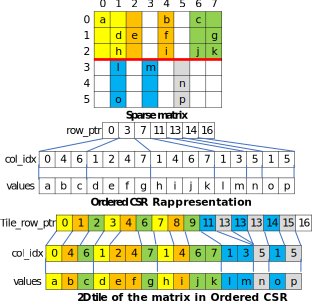
\includegraphics[width=.7\linewidth,keepaspectratio]{csrTilingCSR_only.svg.pdf} 
  \caption[partizionamento 2D CSR]
  {Rappresentazione grafica di un partizionamento 2D di una matrice CSR, \cite{adaptiveTilingSpMM}}
  \decoRule \label{fig:csrTilingCSR_only}
\end{figure}

La suddivisione delle colonne di una matrice CSR, necessaria per il suo partizionamento 2D, 
può essere effettuata \emph{in loco} o mediante sotto matrici CSR separate con una struttura di offest di supporto.

Nel seguito saranno descritte due soluzione che ho realizzato per effettuare l'operazione in oggetto.\\

\subsection{Partizionamento colonne in loco mediante offsets di supporto} 
\label{chSpMMAux:csrColPartitioning}
Per accedere in loco una matrice CSR $M\times N$ in blocchi bidimensionali di $\frac{M}{gridRows}\times\frac{N}{gridCols}$, 
ho realizzato un supporto alla generazione di una matrice di offset $M\times gridCols$, dove l'elemento
$i,j$ è relativo all'inizio della $j$-esima partizione di colonne della $i$-esima riga.\\
\begin{lstlisting}
///OFFSETS COMPUTE FOR COL GROUPS -> O( A.NZ )
for (ulong r=0, j=0;     r<A->M;     j=A->IRP[++r]-OFF_F){
    offsets[ IDX2D(r,0,gridCols) ] = j;  //row's first gc start is costrained
    for (ulong gc=1,gcStartCol;  gc<gridCols;  gc++){
        gcStartCol = UNIF_REMINDER_DISTRI_STARTIDX(gc,_colBlock,_colBlockRem);
        //goto GroupCols start entry,keeping A's nnz entries navigation (idx j)
        while ( j < A->IRP[r+1]-OFF_F &&  A->JA[j]-OFF_F < gcStartCol )  j++;
        offsets[ IDX2D(r,gc,gridCols) ] = j;  //row's gc group startIdx
    }
}
\end{lstlisting}
Nel frammento di codice precedente è possibile vedere come la matrice da partizionare è scansionata
linearmente, salvandone l'indice di colonna corrente ogni volta che 
viene raggiunto o superato l'inizio di un gruppo di colonne.\\

\subsection{Partizionamento colonne mediante sotto-matrici dedicate} \label{chSpMMAux:csrColPartitioningAllocatd}
Un approccio alternativo al precedente è quello di separare i gruppi di colonne della matrice da 
partizionare in sotto matrici separate.
Successivamente è possibile accedere un blocco 2D della matrice originaria partizionando 
le righe (indirizzandole con IRP) di ogni sotto matrice ottenuta.\\
Ho realizzato due implementazioni di quest'approccio,
uno basato sull'uso della struttura ausiliara vista nella sottosezione precedente, 
ed un'altra basata su una scansione diretta della matrice, simile al caso precedente.\\ 

\begin{lstlisting}
for (ulong r=0, j=0;     r<A->M;     j=A->IRP[++r]-OFF_F){
    //navigate column groups inside current row
    for (ulong gc=0,gcEndCol=0,i;  gc<gridCols ;  gc++,j+=i){
        i = 0;  //@i=len current subpartition of row @r to copy
        colPart = colParts + gc;
        colPart->IRP[r] = colPartsLens[gc];	
        gcEndCol += UNIF_REMINDER_DISTRI(gc,_colBlock,_colBlockRem);
        //goto next GroupCols,keeping A's nnz entries navigation ( index j+i )
        while ( j+i < A->IRP[r+1]-OFF_F && A->JA[j+i]-OFF_F < gcEndCol ) i++;
        memcpy(colPart->AS+colPart->IRP[r], A->AS+j, i*sizeof(*A->AS));
        memcpy(colPart->JA+colPart->IRP[r], A->JA+j, i*sizeof(*A->JA));
        
        colPartsLens[gc] += i;
		#ifdef ROWLENS
        colPart->RL[r] = i;
		#endif
    }
}
\end{lstlisting}
Nel frammento di codice precedente è possibile vedere come scansionando la matrice da partizionare,
si associ all'indice corrente l'inizio della partizione di colonne da riempirea(\vvv{j})
e la dimensione (\vvv{i}) della sotto riga attuale.%nella partizione di colonne.
Con queste informazioni è possibile effettuare una \vvv{memcpy} dei \nnz relativi 
\vvv{gc}-esima partizione della \vvv{r}-esima riga della matrice (righe 10-11),
dopo che l'indice di scanzionamento corrente della matrice \vvv{j+i} sia arrivato alla 
fine della sotto riga da copiare.\\

\subsection{Confronto teorico delle due soluzioni}
\begin{itemize}
	\item
	L'approccio basato sulla generazione di sottomatrici per ogni partizione di colonna 
	soffre di un overhead di inizializzazione superiore all'altro dato che 
	oltre che scansionare la matrice per identificarne blocchi di colonne, è necessario effettuarne
	copie in altre zone di memoria.\\
	\item 
	L'approccio basato sulla struttura di indicizzazione ausiliaria applicato alla realizzazione
	del prodotto numerico con partizionamento 2D del lavoro, soffre di una possibile penalità di memoria
	nell'accedere righe consecutive di una stessa partizione, dato che i \nnz relativi non sono 
	contigui in memoria.
\end{itemize}

\section{Verfica correttezza delle implementazioni}
Tutte le implementazioni parallele realizzate per Sp3MM sono state verificate 
mediante un confronto con una matrice risultante ottenuta esternamente o
da una implementazione seriale di riferimento.
In entrambi i casi, il confronto è considerato positivo se c'è una uguaglianza esatta 
tra le dimensioni delle matrici e gli indici degli elementi \nnz (il componente \vvv{JA} del formato CSR)
e se i valori floating point delle matrici sono uguali a meno di una soglia di tolleranza (configarata con $7~10^{-4}$.\\
È importante sottolineare la necessità di effettuare il confronto tra valori \nnz delle matrici con una soglia,
%dato che le rappresentazioni floating-point per i numeri reali sono soggetti ad errori di approssimazione, 
dato che le operazioni tra rappresentazioni floating-point sono soggette ad errori di approssimazione che possono portare 
a risultati diversi in base al sequenziamento delle operazioni effettuate (non prevedibile in una implementazione parallela)
\cite{goldmanFP}

\subsection{implementazione seriale di riferiemento}	\label{implSerialeRiferimento}
L'implementazione seriale di riferimento è stata realizzata con una coppia di operazioni di SpMM
realizzate con un approccio \rowbyrow, in modo molto simile alle implementazioni monodimensionali descritte in \ref{chSpMMNum:part1DGroup}.
A differenza della controparte parallela, l'implementazione seriale gode della grande facilitazione 
di poter scrivere le righe della matrice risultante direttamente nell'output dell'operazione senza una fase simbolica precedente,
data la possibilità di accumulare le lunghezze delle righe calcolate precedentemente alla corrente.\\
\voidLine
Per validare gli output dell'implementazione seriale per alcuni input di piccola dimensione,
è stato effettuato un confronto con una implementazione di riferimento per matrici dense: \vvv{CBLAS} in \url{http://www.netlib.org/blas/},
in seguito ad una trasformazione delle matrici da un formato sparso ad uno denso.\\

\section{Distribuzione uniforme del lavoro tra i thread}	\label{chSpMMAux:UNIF_REMINDER_DISTRI}
Distribuire uniformemente il carico di lavoro tra i thread è un'operazione importante,
che consente di minimizzare il divario tra i tempi di completamento dei vari thread 
e conseguentemente anche il tempo di esecuzione parallelo
(dal momento che è definito con l'istante di terminazione dell'ultimo thread).\\

Algoritmi paralleli basati su strutture sparse sono spesso accumunati da 
un'impossibilità di determinare efficientemente il carico di lavoro di effettivo
relativo ad una partizione dell'input.
Nonostante ciò, può essere utile distribuire il più uniformente possibile ogni partizione 
di dati e iterazioni tra i thread .\\%in assenza di informazioni che consentano di effettuare un partizio
Considerando un input di dimensione $n$ da suddividere tra $t$ threads, avendo\\
$div=\left\lfloor \frac{n}{t}  \right\rfloor ~ rem=n ~mod ~t$,
l'approccio seguito per minimizzare il divario delle partizioni assegnate %a vari thread
è realizzato dalla seguente macro:\\
\verb|#define UNIF_REMINDER_DISTRI(i,div,rem) ((div)+((i)<(rem)?1:0 ))|
dove viene redistribuito il resto della divisione $rem$ tra i thread.\\
